\section{Model Checking}\label{sec:otf}
Programs that use mutual exclusion to protect accesses to shared variables introduce non-determinism as different access orders in the critical sections may lead to different computation graphs. Model checking can be used to enumerate each of these computation graphs. The task parallel language is extended to model mutual exclusion with a new statement: $\textbf{isolated}~s$.
The statement performs $s$ in mutual exclusion of any other isolated statements. The semantics with the computation graph construction is in \figref{fig:isol-semantics}. The isolation is accomplished by creating a new global variable \textit{last} to track the last node in the computation graph belonging to an isolated statement, by adding to the task context a counter initialized to zero to count the number of nested isolated contexts, and with a new keyword for the rewrite rules: \textbf{isolated-end}. 

\begin{figure*}
  \begin{center}
    \mprset{flushleft}
    \begin{mathpar}
     \and
      \inferrule[Isolated]
                {
				  \mathrm{canIsolate(C)} = \mathit{true} \\
                  n^\prime = \mathrm{fresh}() \\
                  N = N \cup \{n^\prime\} \\
                  E = E \cup \{\tuple{n, n^\prime},  \tuple{\mathit{last},n^\prime}\}\\
                }
{C[\tuple{\ell^\prime,S[\textbf{isolated}~s],\vec{r_\delta}^\prime,\vec{r_\omega}^\prime,d^\prime, n, 0}, m] \rightarrow
                  C[\tuple{\ell^\prime,
				   S[s; \textbf{isolated-end}],\vec{r_\delta}^\prime,\vec{r_\omega}^\prime,d^\prime, n^\prime, 1}, m]
                }
\and
      \inferrule[Isolated-Nested]
                {\mathit{iso} > 0 \\
                  \mathit{iso}^\prime = \mathit{iso} + 1
                }
{C[\tuple{\ell^\prime,S[\textbf{isolated}~s],\vec{r_\delta}^\prime,\vec{r_\omega}^\prime,d^\prime, n, \mathit{iso}}, m] \rightarrow
                  C[\tuple{\ell^\prime,
				   S[s; \textbf{isolated-end}],\vec{r_\delta}^\prime,\vec{r_\omega}^\prime,d^\prime, n, \mathit{iso}^\prime}, m]
}
\and
      \inferrule[Isolated-End-Nested]
                {\mathit{iso} > 1 \\
                  \mathit{iso}^\prime = \mathit{iso} - 1
                }
{C[\tuple{\ell^\prime,S[\textbf{isolated-end}],\vec{r_\delta}^\prime,\vec{r_\omega}^\prime,d^\prime, n, \mathit{iso}}, m] \rightarrow
                  C[\tuple{\ell^\prime,
				   S[\textbf{skip}],\vec{r_\delta}^\prime,\vec{r_\omega}^\prime,d^\prime, n, \mathit{iso}^\prime}, m]
                }
\and
      \inferrule[Isolated-End]
                {
                  n^\prime = \mathrm{fresh()}\\
                  \mathit{last} = n \\
                  N = N \cup \{n^\prime\} \\
                  E = E \cup \{\tuple{n, n^\prime}\}
                }
{C[\tuple{\ell^\prime,S[\textbf{isolated-end}],\vec{r_\delta}^\prime,\vec{r_\omega}^\prime,d^\prime, n, 1}, m] \rightarrow
                  C[\tuple{\ell^\prime,
				   S[\textbf{skip}],\vec{r_\delta}^\prime,\vec{r_\omega}^\prime,d^\prime, n^\prime,0}, m]
                }

\end{mathpar}
  \end{center}
  \caption{The transition rules for isolated statements.}
  \label{fig:isol-semantics}
\end{figure*}

Let $\mathrm{canIsolate}(C)$ be a function over configurations to Boolean that returns true for a configuration tree if all the task counters are 0; otherwise it returns false. If no other isolated statements are running, then the \textsc{Isolated} rule increments the task counter to indicate isolation and inserts after the isolated statement $\mathit{s}$ the new \textbf{isolated-end} keyword. The computation graph gets a new node to track accesses in the isolated statement with an appropriate edge from the previous node. A sequencing edge from $\mathit{last}$ is also added so the previous isolated statement happens before this new isolated statement. As a note, $\mathit{last}$ is initialized to an empty node when execution starts. The \textsc{Isolated-Nested} rule simply increments the counter if the task is already in isolation.

The \textsc{Isolated-End-Nested} rule processes the new \textbf{isolated-end} keyword and decrements the counter. When the counter reaches the outer-most isolated context, the \textsc{Isolated-End} rule creates a new node in the computation graph to denote the end of isolation, and it updates $\mathit{last}$ to properly sequence any future isolation. As a note, the on-the-fly data race detection is modified to not reduce sub-graphs with isolation.

Algorithm \ref{algo:isolated} presents a scheduling algorithm to enumerate all computation graphs resulting from isolation for model checking \cite{mercer2015model}. The algorithm considers a simplified state of the program with $\mathtt{Regs}$ being the set of region variables that are shared among the tasks, $\mathtt{Tasks}$ being the set of tasks, $t$ being a task, and $R$ being the set of runnable tasks. The algorithm also implements \emph{sequential semantics}, or depth-first semantics, where only one task runs at a time and that task runs until it waits, completes, or isolates at which time a scheduling choice is made. Sequential semantics are viable by \lemmaref{lem:drf} and \corref{cor:drf} that establish independence in the computation graph and execution schedule in the absence of data races. 

\begin{algorithm}
\caption{Scheduling algorithm for Isolated blocks} \label{algo:isolated}
\begin{algorithmic}[1]
  \Function{schedule}{$t$, $\mathtt{Regs}$, $\mathtt{Tasks}$}
  \State \texttt{loop}:\ ($\mathtt{Regs}$, $\mathtt{Tasks}$) $:=$ \texttt{run}($t$, $\mathtt{Regs}$, $\mathtt{Tasks}$)\label{loc:run}
  \State $s :=$ \texttt{status}($t$)
  \State $R :=$ \texttt{runnable}($\mathtt{Tasks}$)
  \If{ $s =$ ISOLATED}\label{loc:entry:isolated}
  \ForAll{$t_i \in R$}\label{loc:prsched}
  \State \texttt{schedule}($t_i$, $\mathtt{Regs}$, $\mathtt{Tasks}$)
  \EndFor
  \Else
  \State $t_i$ := \texttt{random}($R$)\label{loc:rand}
  \State \texttt{schedule}($t_i$, $\mathtt{Regs}$, $\mathtt{Tasks}$)
  \EndIf
  \EndFunction
\end{algorithmic}
\end{algorithm}


Line 2 updates the region variables and pool of tasks by running task $t$ until it exits, waits, or reaches an \textbf{isolated}-construct. The function \texttt{status} on Line 3 returns the status of the task $t$. On Line 4, the function \texttt{runnable} is used to obtain a list of all the tasks that can be run from the pool of all tasks. If the status of the currently running task $t$ becomes ISOLATED (i.e., the task encounters an \textbf{isolated} construct), the task is preempted and all the tasks that are runnable, including the task that is trying to isolate, are scheduled by the runtime meaning that the model checker considers all ways to interleave the runnable tasks at that point. When the task completes, a new task is randomly selected from the set of runnable tasks.

\begin{comment}
\begin{figure}
  \begin{center}
    \begin{lstlisting}[mathescape=true]
  proc main(var n : int)
  	n := 1;
  	post $r_1 \leftarrow p_1~n~\varepsilon~\{r_1\}~\{r_1\}~\lambda v. n := n + v$;
  	post $r_1 \leftarrow p_2~n~\varepsilon~\{r_1\}~\{r_1\}~\lambda v. n := n + v$;
  	await $r_1$
 proc $p_1$(var n : int)
 	isolated $\texttt{l}(r_1) := n + 1$
 proc $p_2$(var n : int)
	isolated if $(\texttt{l}(r_1) = n)$ then
	  	post $r_1 \leftarrow p_3~n~\varepsilon~\{r_1\}~\{r_1\}~\lambda v. n := n + v$;
	else
		$\texttt{l}(r_1) := n - 1$
 proc $p_3$(var n : int)
	$\texttt{l}(r_1) := n+2$
\end{lstlisting}
  \end{center}
%  \vspace{-1em}
  \caption{Parallel Program with Mutual exclusion.}
%  \vspace{-1em}
  \label{fig:hj-isolated}
\end{figure}

\begin{figure}
  \centering
  \subfigure[p2 runs before p1.]{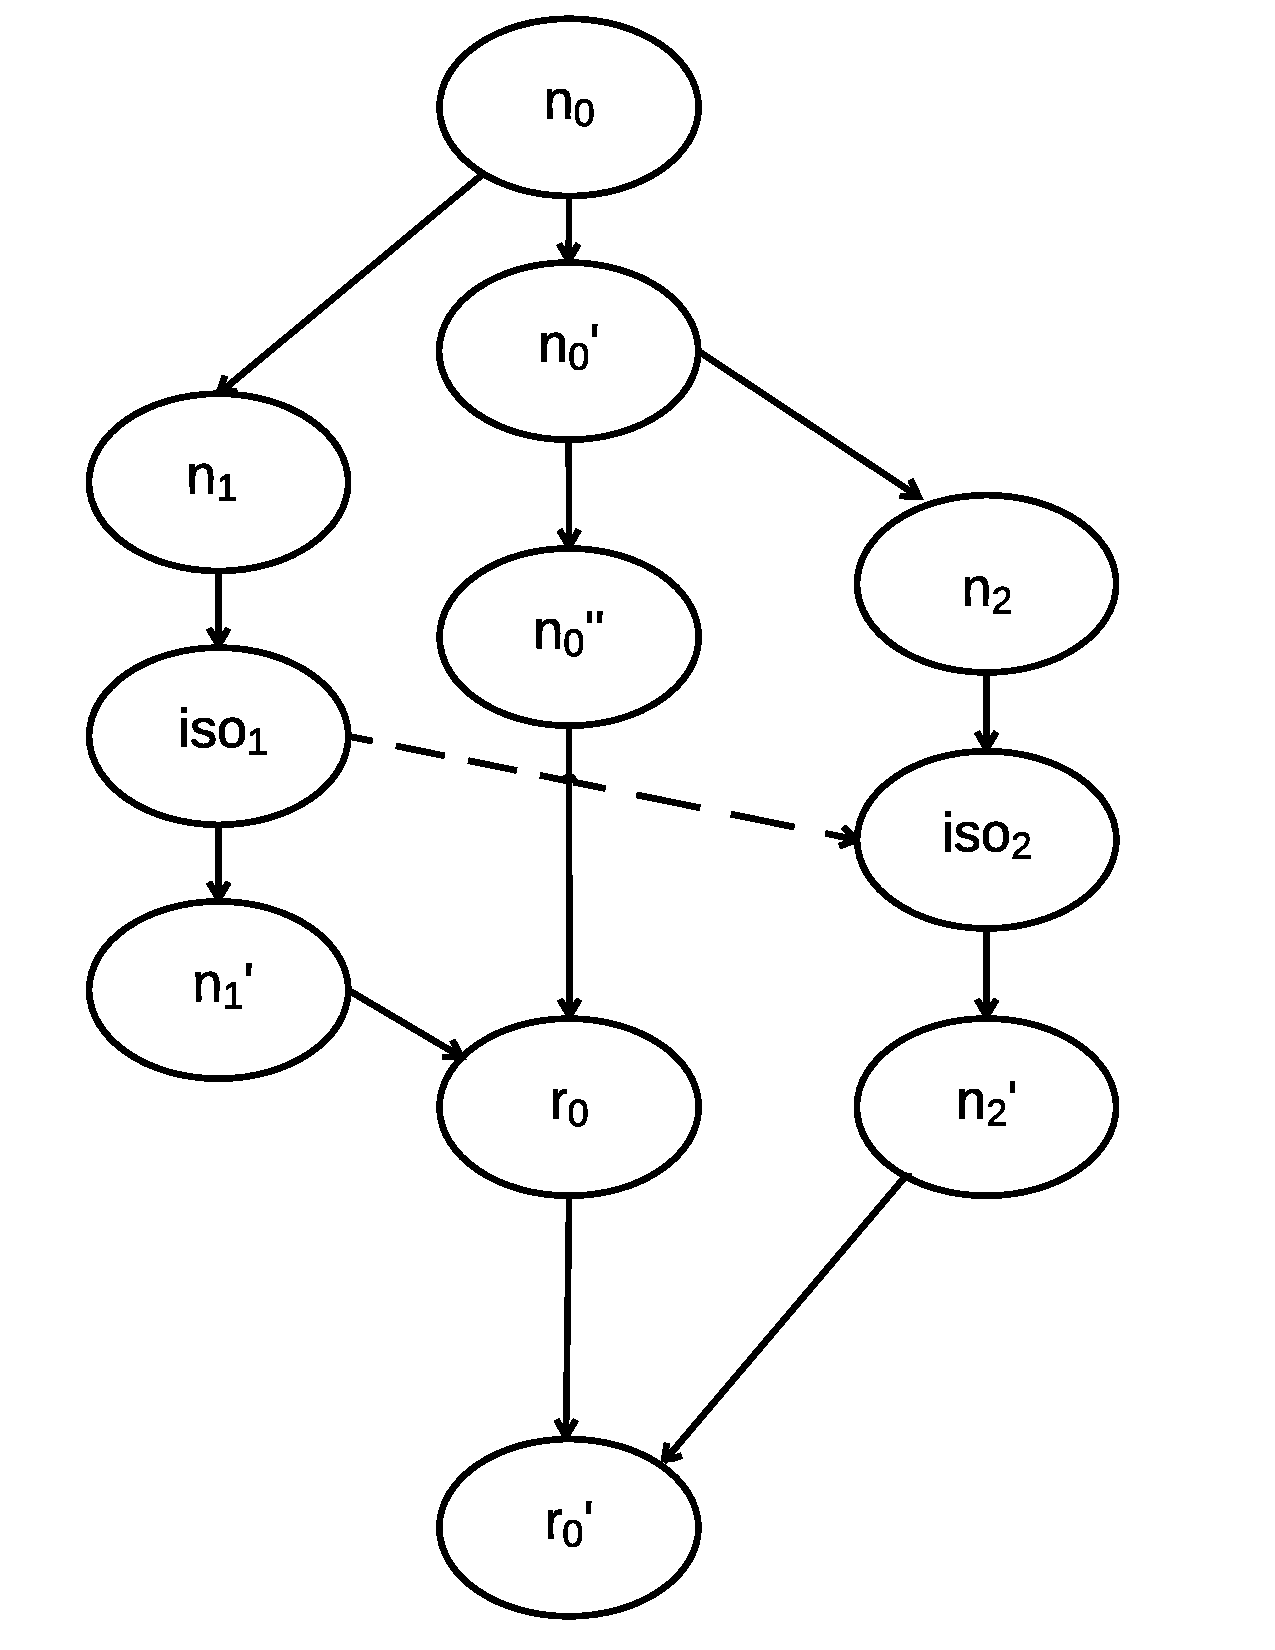
\includegraphics[scale=0.2]{../figs/Fig5-a.pdf}}
  \subfigure[p1 runs before p2.]{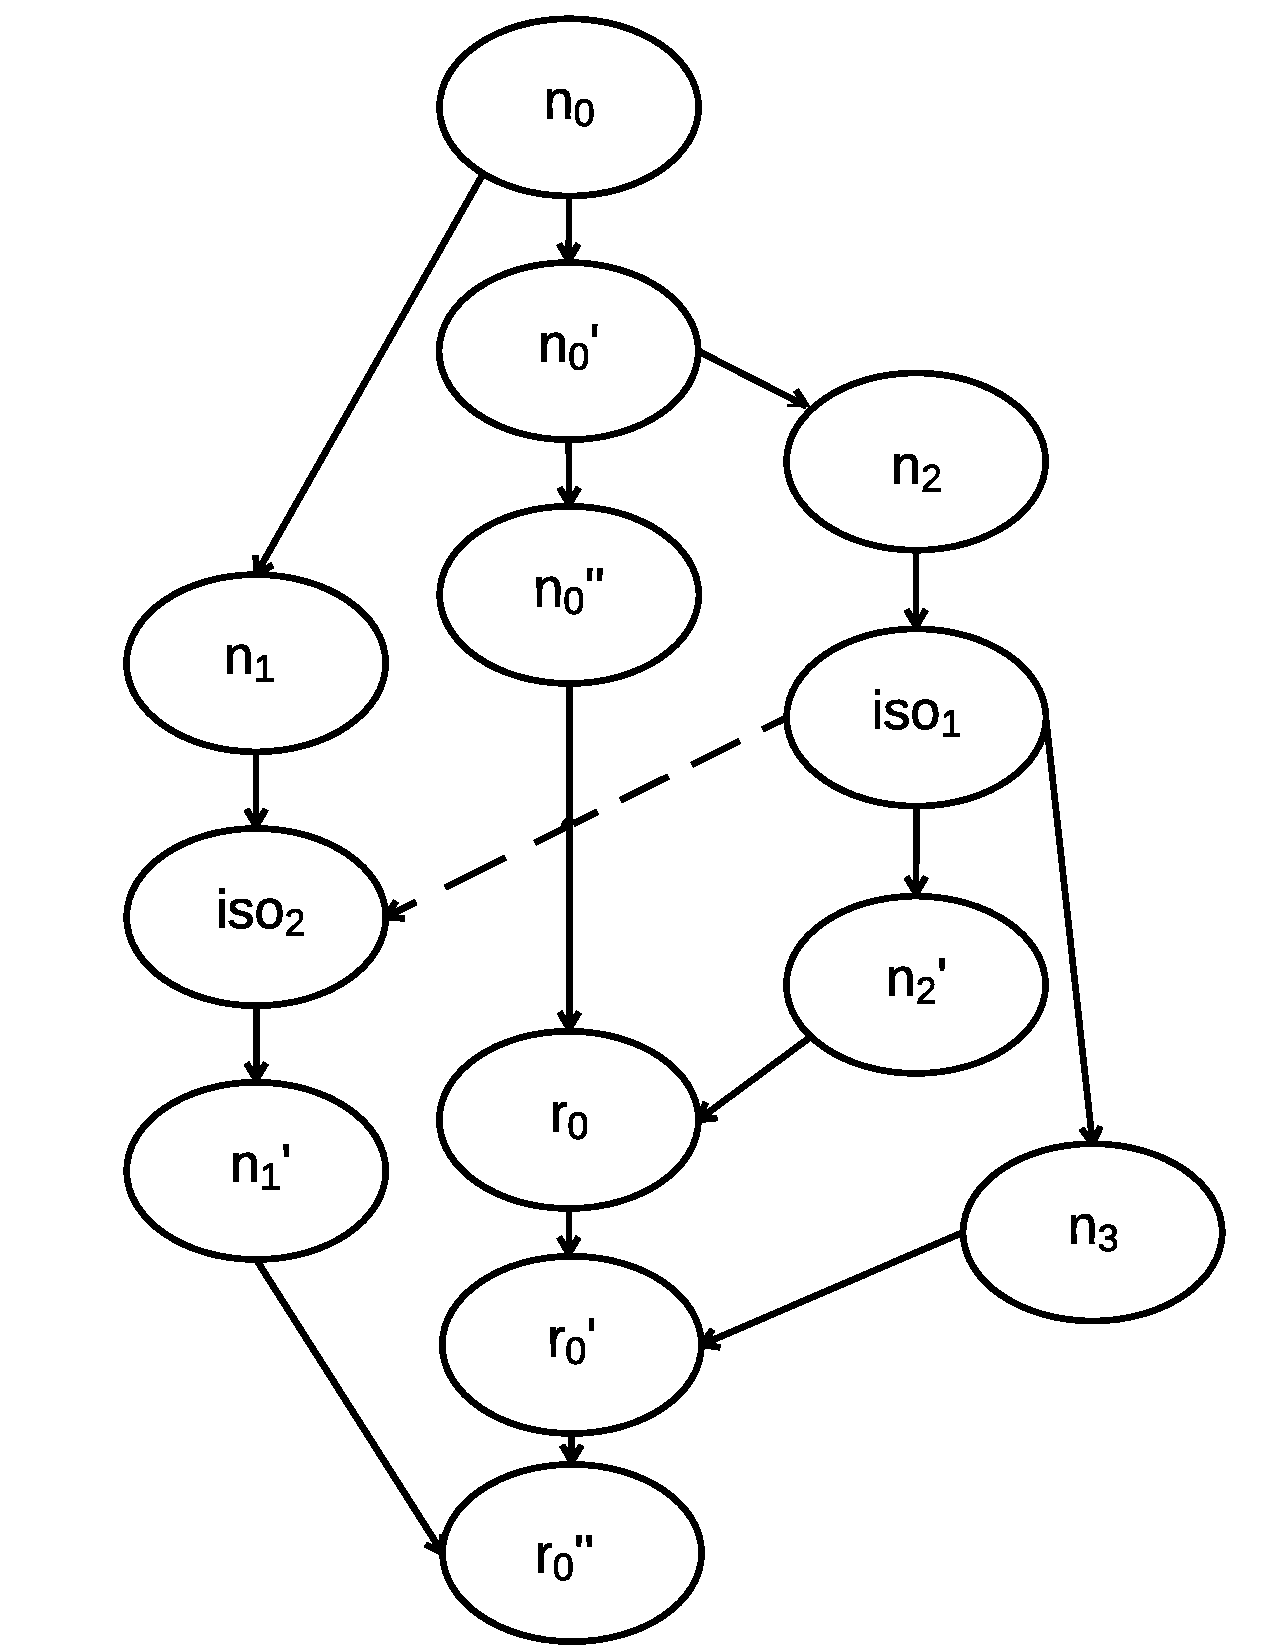
\includegraphics[scale=0.2]{../figs/Fig5-b.pdf}}
  \caption{Computation graphs of example in \figref{fig:hj-isolated}}
%  \vspace{-1em}
   \label{fig:cg-isolated}
\end{figure}

For the example in \figref{fig:hj-isolated}, two different computation graph structures can be formed based on the order of execution of isolated blocks. The computation graphs are shown in \figref{fig:cg-isolated}. If the scheduler runs the isolated section of task $t_1$ first, the computation graph in \figref{fig:cg-isolated}(a) is formed. Task $t_1$ changes the values of shared variable $r_1$ to 2. Hence, when task $t_2$ executes its isolated section, the if-condition fails and an additional task is not spawned by $t_2$. If the scheduler runs task $t_2$ first, the computation graph of \figref{fig:cg-isolated}(b) is formed. In this schedule, task $t_2$ executes its isolated section first. Since the value of variable $r_1$ is 1, the if-condition is met and a new task is created by $t_2$.
\end{comment}

\begin{theorem}
\algoref{algo:isolated} creates all possible computation graphs due isolation. 
%\algoref{algo:drd} is sound and complete for structured parallel programs with mutual exclusion.
\end{theorem}

Model checking enumerates and checks each possible computation graph from the program to determine if it is data-race free. Since every graph is considered, and the technique is sound and complete, only programs that are truly data-race free are accepted.

\begin{comment}
\begin{proof}
%Theorem \ref{thm:strcutured-par-progs} states that Algorithm \ref{algo:drd} is sound and complete for structured parallel programs that do not contain isolated sections. If mutual exclusion is present, Algorithm \ref{algo:drd} does not remain sound since different computation graph structures can be formed for such programs. Algorithm \ref{algo:isolated} helps to enumerate all such computation graph structures. Therefore, the data race detection using Algorithm \ref{algo:drd} becomes sound and complete when it is used along with Algorithm \ref{algo:isolated} for structured parallel programs that have mutual exclusion.
From \thmref{thm:strcutured-par-progs} and \algoref{algo:isolated}, \algoref{algo:drd} is sound and complete for structured parallel programs with mutual exclusion.
\end{proof}
\end{comment}
